\documentclass[tikz,border=3pt]{standalone}
\usepackage[T1]{fontenc}
\usepackage{lmodern,amsmath,amssymb}
\usetikzlibrary{arrows.meta,calc}
\newcommand{\Ssys}{\mathcal{S}}
\newcommand{\Env}{\mathcal{E}}
\newcommand{\Frag}{\mathcal{F}}
\newcommand{\Rem}{\mathcal{R}}
\begin{document}
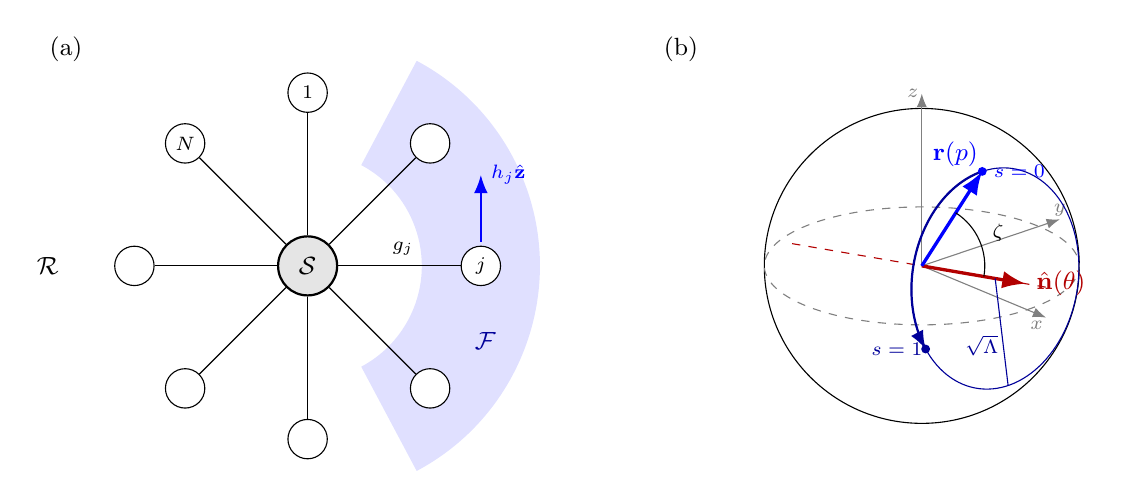
\begin{tikzpicture}[
        >=Latex,
        witness/.style={circle,draw,fill=white,minimum size=5mm,inner sep=0pt,font=\scriptsize},
        system/.style={circle,draw,thick,fill=gray!20,minimum size=7.5mm,inner sep=0pt,font=\small},
        every node/.style={font=\small}
    ]
    % ---------------- panel (a): star geometry ----------------
    \begin{scope}
        \node[anchor=west] at (-3.4,2.75) {(a)};
        % fragment shading, drawn first so nodes sit on top
        \fill[blue!12] (62:1.45) arc (62:-62:1.45) -- (-62:2.95) arc (-62:62:2.95) -- cycle;
        \node[blue!60!black] at (-23:2.45) {$\Frag$};
        \node at (180:3.3) {$\Rem$};
        \node[system] (S) at (0,0) {$\Ssys$};
        \foreach \ang/\name/\lab in {90/W1/{1},45/W2/{},0/W3/{$j$},-45/W4/{},-90/W5/{},-135/W6/{},180/W7/{},135/W8/{$N$}}{
            \node[witness] (\name) at (\ang:2.2) {\lab};
            \draw (S) -- (\name);
        }
        \node[font=\scriptsize] at ($(S)!0.55!(W3)+(0,0.22)$) {$g_j$};
        \draw[->,thick,blue] ($(W3.north)+(0,0.05)$) -- ++(0,0.85)
            node[right,font=\scriptsize] {$h_j\hat{\mathbf z}$};
    \end{scope}
    % ---------------- panel (b): Bloch-sphere geometry ----------------
    \begin{scope}[shift={(7.8,0)}]
        \node[anchor=west] at (-3.4,2.75) {(b)};
        \def\R{2.0}
        \pgfmathsetmacro{\pbeta}{35}    % polar angle of r from z
        \pgfmathsetmacro{\ptheta}{10}   % C-INOT angle from x
        % orthographic projection: azimuth \Ad about z, elevation \Ae; silhouette is the circle of radius R
        \pgfmathsetmacro{\Ad}{48}
        \pgfmathsetmacro{\Ae}{22}
        \pgfmathsetmacro{\uxx}{cos(\Ad)}
        \pgfmathsetmacro{\uxy}{sin(\Ad)}
        \pgfmathsetmacro{\wxx}{-sin(\Ae)*sin(\Ad)}
        \pgfmathsetmacro{\wxy}{sin(\Ae)*cos(\Ad)}
        \pgfmathsetmacro{\wxz}{cos(\Ae)}
        \draw[thin] (0,0) circle (\R);
        % equator (xy plane)
        \draw[thin,dashed,gray] plot[domain=0:360,samples=120,variable=\t]
            ({\R*(\uxx*cos(\t)+\uxy*sin(\t))},{\R*(\wxx*cos(\t)+\wxy*sin(\t))});
        % axes
        \draw[->,gray] (0,0) -- ({1.18*\R*\uxx},{1.18*\R*\wxx}) node[below left,font=\scriptsize,inner sep=1pt] {$x$};
        \draw[->,gray] (0,0) -- ({1.18*\R*\uxy},{1.18*\R*\wxy}) node[above,font=\scriptsize,inner sep=1pt] {$y$};
        \draw[->,gray] (0,0) -- (0,{1.18*\R*\wxz}) node[left,font=\scriptsize,inner sep=1pt] {$z$};
        % C-INOT axis n(theta) in the xz plane
        \pgfmathsetmacro{\nX}{\R*\uxx*cos(\ptheta)}
        \pgfmathsetmacro{\nY}{\R*(\wxx*cos(\ptheta)+\wxz*sin(\ptheta))}
        \draw[dashed,red!70!black] ({-1.25*\nX},{-1.25*\nY}) -- ({1.25*\nX},{1.25*\nY});
        \draw[->,very thick,red!70!black] (0,0) -- (\nX,\nY) node[right] {$\hat{\mathbf n}(\theta)$};
        % initial Bloch vector r(p) in the xz plane
        \pgfmathsetmacro{\rX}{\R*\uxx*sin(\pbeta)}
        \pgfmathsetmacro{\rY}{\R*(\wxx*sin(\pbeta)+\wxz*cos(\pbeta))}
        \coordinate (r) at (\rX,\rY);
        \draw[->,very thick,blue] (0,0) -- (r) node[above left,inner sep=1pt] {$\mathbf r(p)$};
        % angle between r and n, drawn in the projected plane
        \pgfmathsetmacro{\angn}{atan2(\nY,\nX)}
        \pgfmathsetmacro{\angr}{atan2(\rY,\rX)}
        \draw[thin] (\angn:{0.4*\R}) arc (\angn:\angr:{0.4*\R});
        \node[font=\scriptsize,inner sep=1pt] at ({(\angn+\angr)/2}:{0.53*\R}) {$\zeta$};
        % conditional trajectory of the s=1 branch: rotation of r about n
        \pgfmathsetmacro{\sa}{sin(\pbeta+\ptheta)}
        \pgfmathsetmacro{\ca}{cos(\pbeta+\ptheta)}
        \pgfmathsetmacro{\px}{\sa*cos(\ptheta)}
        \pgfmathsetmacro{\pz}{\sa*sin(\ptheta)}
        \pgfmathsetmacro{\ux}{sin(\pbeta)-\px}
        \pgfmathsetmacro{\uz}{cos(\pbeta)-\pz}
        % point on the circle: x = px + ux cos t, y = -ca sin t, z = pz + uz cos t
        \draw[thin,blue!60!black] plot[domain=0:360,samples=120,variable=\t]
            ({\R*(\uxx*(\px+\ux*cos(\t)) - \uxy*\ca*sin(\t))},
             {\R*(\wxx*(\px+\ux*cos(\t)) - \wxy*\ca*sin(\t) + \wxz*(\pz+\uz*cos(\t)))});
        \draw[->,thick,blue!60!black] plot[domain=0:115,samples=60,variable=\t]
            ({\R*(\uxx*(\px+\ux*cos(\t)) - \uxy*\ca*sin(\t))},
             {\R*(\wxx*(\px+\ux*cos(\t)) - \wxy*\ca*sin(\t) + \wxz*(\pz+\uz*cos(\t)))});
        \coordinate (c) at ({\R*(\uxx*\px)},{\R*(\wxx*\px+\wxz*\pz)});
        \coordinate (rone) at
            ({\R*(\uxx*(\px+\ux*cos(115)) - \uxy*\ca*sin(115))},
             {\R*(\wxx*(\px+\ux*cos(115)) - \wxy*\ca*sin(115) + \wxz*(\pz+\uz*cos(115)))});
        % radius of the conditional circle, drawn to the point opposite r
        \coordinate (rtwo) at ({\R*(\uxx*(\px-\ux))},{\R*(\wxx*(\px-\ux) + \wxz*(\pz-\uz))});
        \draw[thin,blue!60!black] (c) -- (rtwo)
            node[midway,anchor=north east,font=\scriptsize,inner sep=1pt] {$\sqrt{\Lambda}$};
        \fill[blue] (r) circle (1.6pt);
        \node[blue,anchor=west,xshift=3pt,font=\scriptsize,inner sep=1pt] at (r) {$s=0$};
        \fill[blue!60!black] (rone) circle (1.6pt);
        \node[blue!60!black,left,font=\scriptsize,inner sep=1pt] at (rone) {$s=1$};
    \end{scope}
    \end{tikzpicture}
\end{document}
